\section{Implementation of Model Fragmentation}
\label{sec:implemention}

In this section, we present the EMF based persistence framework EMFFrag~\cite{EMFFragProject} which implements the presented meta-model based fragmentation strategy (refer to section~\ref{sec:fragmentation}).

\tinyparagraph{Design goal}
The main goal in our implementation is to (re)use EMF resource as much as possible. EMF resources already provide many required functionalities: they realize partial model persistence, resources manage inter-resource references through proxies, resources lazy-load, they can be added and deleted, and objects can be moved between resources. EMFFrag extends the existing implementations of EMF resources. EMFFrag could be realized with a very small code base of less than 800 lines of code.

\begin{figure}[t]
  \centering
  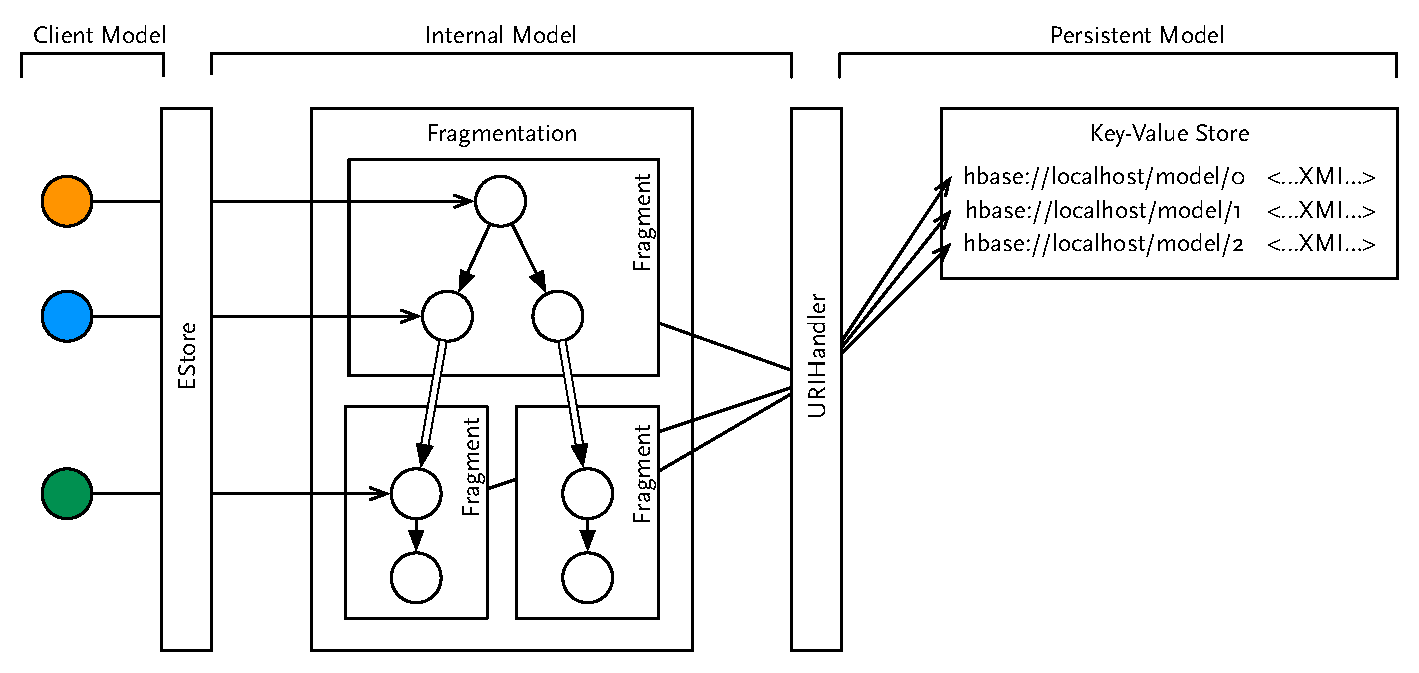
\includegraphics[width=0.75\linewidth]{figures/simpleArchitecture}
  \caption{EMFFrag partially loads a persisted model as internal model of dynamic EMF objects and exposes the model as client model via EMF generated model code with feature delegation.}
  \label{fig:architecture}
	%\vspace*{-2.0ex}
\end{figure}

\tinyparagraph{Underlying key-value store}
EMFFrag uses a simple interface that abstracts from concrete key-value stores. We provide an implementation for HBase (this was used for all measurements in this paper). EMFFrag implements EMF's \texttt{URIHandler} interface to realize key-value store values as resources. Each fragmented model is stored in its own table.

\tinyparagraph{Fragments and fragmentation} EMF \texttt{XMIResource}s are used as fragments and \texttt{ResourceSet}s act as fragmentations. The model is internally realized as a purely dynamic (no generated sources) EMF model.

\tinyparagraph{Transparent load and unload of fragments}
Fragments, Fragmentations, and internal model are hidden from clients (ref. to Fig.~\ref{fig:architecture}). Clients use the model through the usual EMF generated interfaces and classes. Those are configured with reflective feature delegation to an \texttt{EStore}~(\cite{emf2009} explains the concept). 
EMFFrag's \texttt{EStore} implementation simply delegates all calls to internal objects. If necessary, it creates an internal object for each client created object, and a client object for each internal object. Client objects hold references to their internal counterparts. Fragments manage client objects that correspond to the internal objects they contain via Java's \emph{weak references}. When clients loose all strong references to a fragment's contents,  the JVM collects the client objects as garbage (despite existing weak references) and notifies the owning fragment. Thus, fragments know if clients hold references to their objects, and they can safely unload once no more client reference to their contents exist.

\tinyparagraph{Inter-fragment containment references}
Client model classes have to be generated with enabled containment proxies (see~\cite{emf2009}) to allow containment references between resources (i.e. fragments). Users can use EMF Ecore annotation to mark containment reference features as inter-fragment features.
When EMFFrag's \texttt{EStore} implementation delegates a call that manipulates an inter-fragment containment feature, it creates or deletes fragments accordingly and puts objects into their respective fragments.

\tinyparagraph{Inter-fragment cross references}
EMF persists references between XMI resources with URIs. The first part of an URI identifies the resource (i.e. the fragment within a key-value store). The second URI part (URI fragment part) identifies the referenced object within the containing resource. For all inter-fragment containment references and for cross references within a fragment EMF's default \emph{intrinsic ID's}~\cite{emf2009} are used.

Intrinsic IDs are similar to XPath expressions and identify an object via its position in the containment hierarchy. Intrinsic IDs cannot be used for inter-fragment cross references: when an object is moved, its intrinsic ID (URI fragment) changes and all persisted referencing object use invalid URIs. For this reason EMFFrag uses model-wide unique \emph{extrinsic IDs} (an existing EMF functionality). EMFFrag maintains a secondary index (i.e. another table in the key-value store) that maps extrinsic IDs to respective intrinsic IDs. When an object moves this entry is updated and all cross-references are updated automatically. Extrinsic IDs and secondary index are only maintained for objects that are actually cross referenced from another fragment to keep the index small. 